\documentclass[10pt]{article}
\usepackage{icmlko}

\icmlmeta{IP 파운데이션 월드모델}{76}{시간을 갈랐더니 값을 안 치렀다}{배선은 닫혔고, 처음으로 과거만으로 미래 팝업 쉰아홉 건을 예측했다}

\begin{document}

\twocolumn[
\icmlheader

\begin{abstract}
노트 75가 애니 배선 하나로 $+$0.068을 얻었으므로 \textbf{여덟 도메인 전부를
앙상블 자로 다시 돌렸다} --- 후보 \textbf{92개}. 결과는 빈손이다. 최선이 애니
미디어 투입을 더빙으로 바꾸는 $\Delta+$0.0027이고 구간 반폭($\pm$0.011)의 4분의
1이다. \textbf{배선은 닫혔다.} 노트 75에서 사라진 두 셀(게임$\leftrightarrow$애니)도
게임 매장 축을 켜서 살릴 수 있는데 $\Delta-$0.0110이라 값을 안 한다.
그래서 본론은 다른 것이다. \textbf{노트 13부터 일흔다섯까지 모든 수치가 시간을
안 갈랐다.} 붓스트랩이 연도 층화이긴 했지만 그것은 표본 변동을 재는 장치이지
``과거로 미래를 맞히는가''를 재는 장치가 아니다. 시점 $T$를 정하고 \textbf{출처를
$T$ 이전으로 자른 뒤 대상의 $T$ 이후 레코드로만} 평가했다. \textbf{자르는 값이
거의 없다} --- 여덟 대상 평균이 시점 2024에서 $+$0.3253$\to+$0.3395, 2025에서
$+$0.3080$\to+$0.3273으로 오히려 \emph{올랐고} 2026에서 $+$0.2864$\to+$0.2841로
같다. 팝업이 특히 좋다 --- \textbf{2025년 이후에 연 팝업 59건을, 2025년 이전
데이터만으로, $\rho=+$0.5212 {[}$+$0.253, $+$0.715{]}로 순위 매긴다.} 상위 20\%가
872명, 하위 20\%가 115명으로 \textbf{7.55배}다(구간 {[}1.78, 14.52{]}). 처음으로
``예측''이라 부를 수 있는 수치다.
\end{abstract}
]

\begin{figure*}[t]
\centering
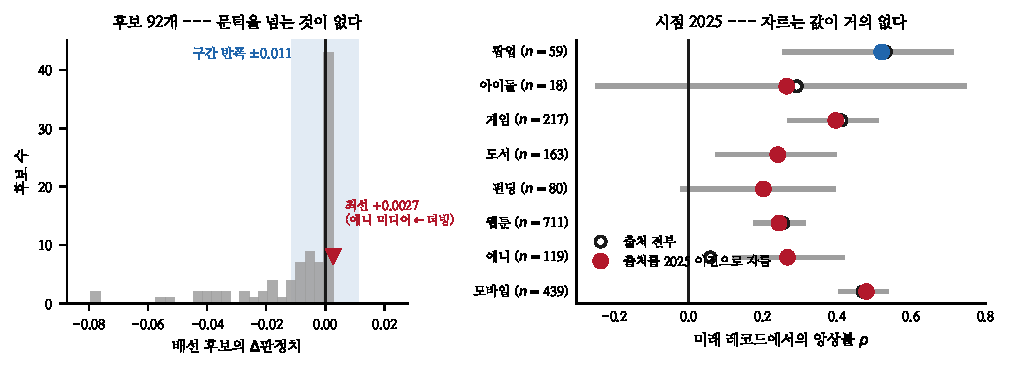
\includegraphics[width=\textwidth]{figs/prosp.pdf}
\caption{왼쪽 --- 배선 후보 92개의 $\Delta$판정치. 오른쪽 --- 시점 2025의 미래
평가(속 빈 표식이 출처 전부).}
\end{figure*}

\section{배선은 닫혔다}

노트 75가 애니 하나에서 $+$0.068을 얻었으므로 나머지도 있으리라 봤다. 여덟
도메인의 후보를 전부 돌렸다 --- 슬롯마다 등록된 후보 열, 합쳐 92개.

\begin{table}[t]
\centering\tsize
\caption{$\Delta$판정치 상위 다섯. 구간 반폭은 0.011이다.}
\begin{tabular}{lllr}
\toprule
도메인 & 슬롯 & 후보 & $\Delta$ \\
\midrule
애니 & 미디어 투입 & 더빙 & $+$0.0027 \\
웹툰 & 매장 노출도 & 작가 수 & $+$0.0014 \\
웹툰 & 매장 노출도 & 요일 수 & $+$0.0011 \\
애니 & 미디어 투입 & 독점/오리지널 & $+$0.0009 \\
웹툰 & 미디어 투입 & 작가 수 & $+$0.0001 \\
\bottomrule
\end{tabular}
\end{table}

\claimx{현재 배선은 앙상블 자에서 국소 최적이다. 후보 92개 중 어느 것도 구간
반폭의 4분의 1을 못 넘는다. 배선은 더 이상 지렛대가 아니다.}{후보 풀이 내가
등록한 것뿐이다. 새 물리량을 수집해 후보에 넣으면 다를 수 있다 --- 노트 45가
같은 결론을 냈다가 도메인 추가로 뒤집었다.}

노트 75에서 애니가 굿즈 규모를 잃어 게임과 공통 축이 하나뿐이 되고 두 셀이
사라졌다. 게임 매장 축(퍼블리셔 이력)을 켜면 살아나는데 $\Delta-$0.0110이다.
\textbf{두 셀보다 게임 축 하나가 더 비싸다.} 54셀로 둔다.

\section{시간을 갈랐다}

\begin{quote}\fontsize{9.5}{11.5}\selectfont
\textbf{지금까지 모든 수치가 시간을 안 갈랐다.} 출처 도메인의 2026년 레코드로
학습한 회귀가 2025년 팝업을 맞히는 것이 평가였다. 제품은 그렇게 안 쓰인다 ---
쓰이는 방식은 하나다. \emph{지금까지 쌓인 것으로 배워서 아직 안 연 팝업을 맞힌다.}
\end{quote}

규약을 셋으로 정했다. 시점 $T$를 정하고, \textbf{출처는 $T$ 이전 레코드만}
쓰고, \textbf{대상은 $T$ 이후 레코드로만} 평가한다. 미래 집합이 작아 $\rho$가
흔들리므로 \textbf{같은 미래 집합에서 두 번} 잰다 --- 출처를 자른 것과 안 자른
것. 차이가 ``미래를 못 보는 값''이다.

\begin{table}[t]
\centering\tsize
\caption{여덟 대상 평균 앙상블 $\rho$.}
\begin{tabular}{lrrr}
\toprule
시점 & 출처 전부 & 출처를 자름 & 차이 \\
\midrule
2024 & $+$0.3253 & $+$0.3395 & $+$0.0142 \\
2025 & $+$0.3080 & $+$0.3273 & $+$0.0193 \\
2026 & $+$0.2864 & $+$0.2841 & $-$0.0023 \\
\bottomrule
\end{tabular}
\end{table}

\claimx{출처를 과거로 자르는 값이 거의 없다 --- 세 시점 중 둘에서 오히려
올랐다. 이 모형은 시간을 갈라도 성립한다.}{자른 뒤에도 출처 표본이 커서
(웹툰 1,000건대, 모바일 500건대) 손실이 안 보이는 것일 수 있다. 아이돌처럼
작은 출처는 자르면 44건이 된다.}

\section{팝업 --- 아직 안 연 것을 맞힌다}

\begin{table}[t]
\centering\tsize
\caption{팝업. 미래 레코드에서만 평가.}
\begin{tabular}{lrrl}
\toprule
시점 & 미래 $n$ & $\rho$(과거만) & 95\% 구간 \\
\midrule
2024 & 74 & $+$0.4596 & $[+0.251, +0.631]$ \\
\textbf{2025} & \textbf{59} & \textbf{$+$0.5212} & $[+0.253, +0.715]$ \\
2026 & 19 & $+$0.4246 & $[-0.132, +0.783]$ \\
\bottomrule
\end{tabular}
\end{table}

시점 2025가 가장 좋다 --- \textbf{2025년 이후에 연 팝업 59건을 2025년 이전
데이터만으로 $\rho=+$0.5212로 줄 세운다.} 전체 데이터로 잰 $+$0.448보다 높다.
2026 시점은 미래가 19건뿐이라 구간이 0을 포함한다.

\begin{table}[t]
\centering\tsize
\caption{제품 수치 --- 미래 팝업의 예측 상하위 20\% 일평균 방문자.}
\begin{tabular}{lrrrl}
\toprule
시점 & $n$ & 상위 & 하위 & 배수 \\
\midrule
2024 & 74 & 877명 & 164명 & 5.34 $[2.08, 10.77]$ \\
\textbf{2025} & 59 & 872명 & 115명 & \textbf{7.55} $[1.78, 14.52]$ \\
\bottomrule
\end{tabular}
\end{table}

노트 71이 배수의 구간을 처음 붙였고 여전히 넓다. 그래도 \textbf{이번 배수는
미래 레코드에서 나왔다} --- 노트 58 이후 처음으로 ``예측''이라 부를 수 있는
수치다.

\begin{quote}\fontsize{9.5}{11.5}\selectfont
제품 문장을 고쳐 쓴다. \textbf{2025년 이전 데이터만 가지고, 그 뒤에 연 팝업
59건의 순위를 $\rho=+$0.52로 맞혔다.} 배수는 7.55배지만 구간이 {[}1.78,
14.52{]}라 여전히 \emph{몇 명 올지}는 약속 못 한다. \emph{어느 기획을 먼저
밀지}는 이제 미래 데이터로 검증됐다.
\end{quote}

\section{한계}

\begin{itemize}[leftmargin=1.1em,itemsep=0.15em]
\item 대상의 인자 공간을 미래 레코드 \emph{전체}로 만든다. 팝업 축은 기획
      단계에 정해지므로 라벨 누출은 아니지만, 여러 건을 한꺼번에 보는
      전도적 가정이 남는다. 한 건씩 예측하는 것과는 다르다.
\item 시점 셋만 봤다. 팝업 표본이 2023--2026이라 더 못 자른다.
\item 배선과 축 선택은 \emph{전체} 데이터로 골랐다. 시간을 가른 것은 회귀
      학습과 평가뿐이고, 설계 결정에는 미래가 들어가 있다.
\item 애니가 시점 2024 · 2025에서 자를 때 크게 좋아진다($+$0.18, $+$0.21).
      이유를 안 봤다.
\item 배수 구간이 여전히 팝업 표본 크기에 지배된다(노트 75).
\end{itemize}

\section{다음}

\begin{enumerate}[leftmargin=1.3em,itemsep=0.15em]
\item \textbf{설계 결정도 시간을 가른다} --- 배선과 축을 $T$ 이전 데이터로만
      고르고 $T$ 이후로 평가한다. 지금 남은 가장 큰 누출이다.
\item 한 건씩 예측하는 규약 --- 대상 인자 공간을 과거 레코드로 만들고 새 기획
      하나를 투영한다. 전도적 가정을 없앤다.
\item 아홉째 도메인 --- 배선이 닫혔으므로 남은 지렛대는 이것뿐이다.
\item 애니가 자를 때 좋아지는 이유.
\end{enumerate}

\vspace{0.6em}
\hrule height 0.3pt
\vspace{0.5em}
{\footnotesize
\textbf{참고문헌}\\[0.3em]
Bergmeir, C., Benitez, J. M. (2012). On the use of cross-validation for time
series predictor evaluation. \emph{Information Sciences}, 191, 192--213.\\[0.15em]
Kaufman, S., Rosset, S., Perlich, C. (2012). Leakage in data mining.
\emph{ACM TKDD}, 6(4), 1--21.\\[0.15em]
Cawley, G. C., Talbot, N. L. C. (2010). On over-fitting in model selection and
subsequent selection bias in performance evaluation. \emph{JMLR}, 11, 2079--2107.\\[0.15em]
Efron, B., Tibshirani, R. J. (1993). \emph{An Introduction to the Bootstrap}.
Chapman \& Hall.\\[0.15em]
Ben-David, S. et al. (2010). A theory of learning from different domains.
\emph{Machine Learning}, 79(1--2), 151--175.
}

\end{document}
